\subsection{Energieübertragung}\label{sec:energieuebertragung}

Die Funktionsweise der Induktiven Ladung wird veranschaulicht dargestellt und erläutert mit Schema, Simulation und ggf. weitere Abbildungen.


Im Joscha sin Teil
\newline
\newline
\newline
\newline
\newline







Nachdem die gesamte induktive Ladeschaltung beschrieben wurde, folgt ein Prototyp für die Ladestation. Diese implementiert die gesamte primäre induktive Ladeschaltung, welche bereits im oberen Teil beschrieben wurde. Für den Prototypen wurde eine .stl Datei erstellt welche mit einem 3D-Drucker gedruckt wurde. Wichtig ist hierbei die Erwähnung, dass es sich bei nachfolgende Abbildungen \ref{fig:Prototyp Front} bis \ref{fig:Prototyp Down} nur um Prototypen handelt und nicht um definitive Ladestationen. Da die Ladestation für Versuchszwecke bereits erstellt wurde und für Implementierung des Primärkreislaufes der Induktiv-Ladeschaltung wurde das Design so gewählt, dass nur ein Dojo geladen werden kann. Dies würde in einem weiteren Schritt auf mehrere Ladeaussparungen erweitert werden. 

\begin{figure}[H]
	\begin{center}
		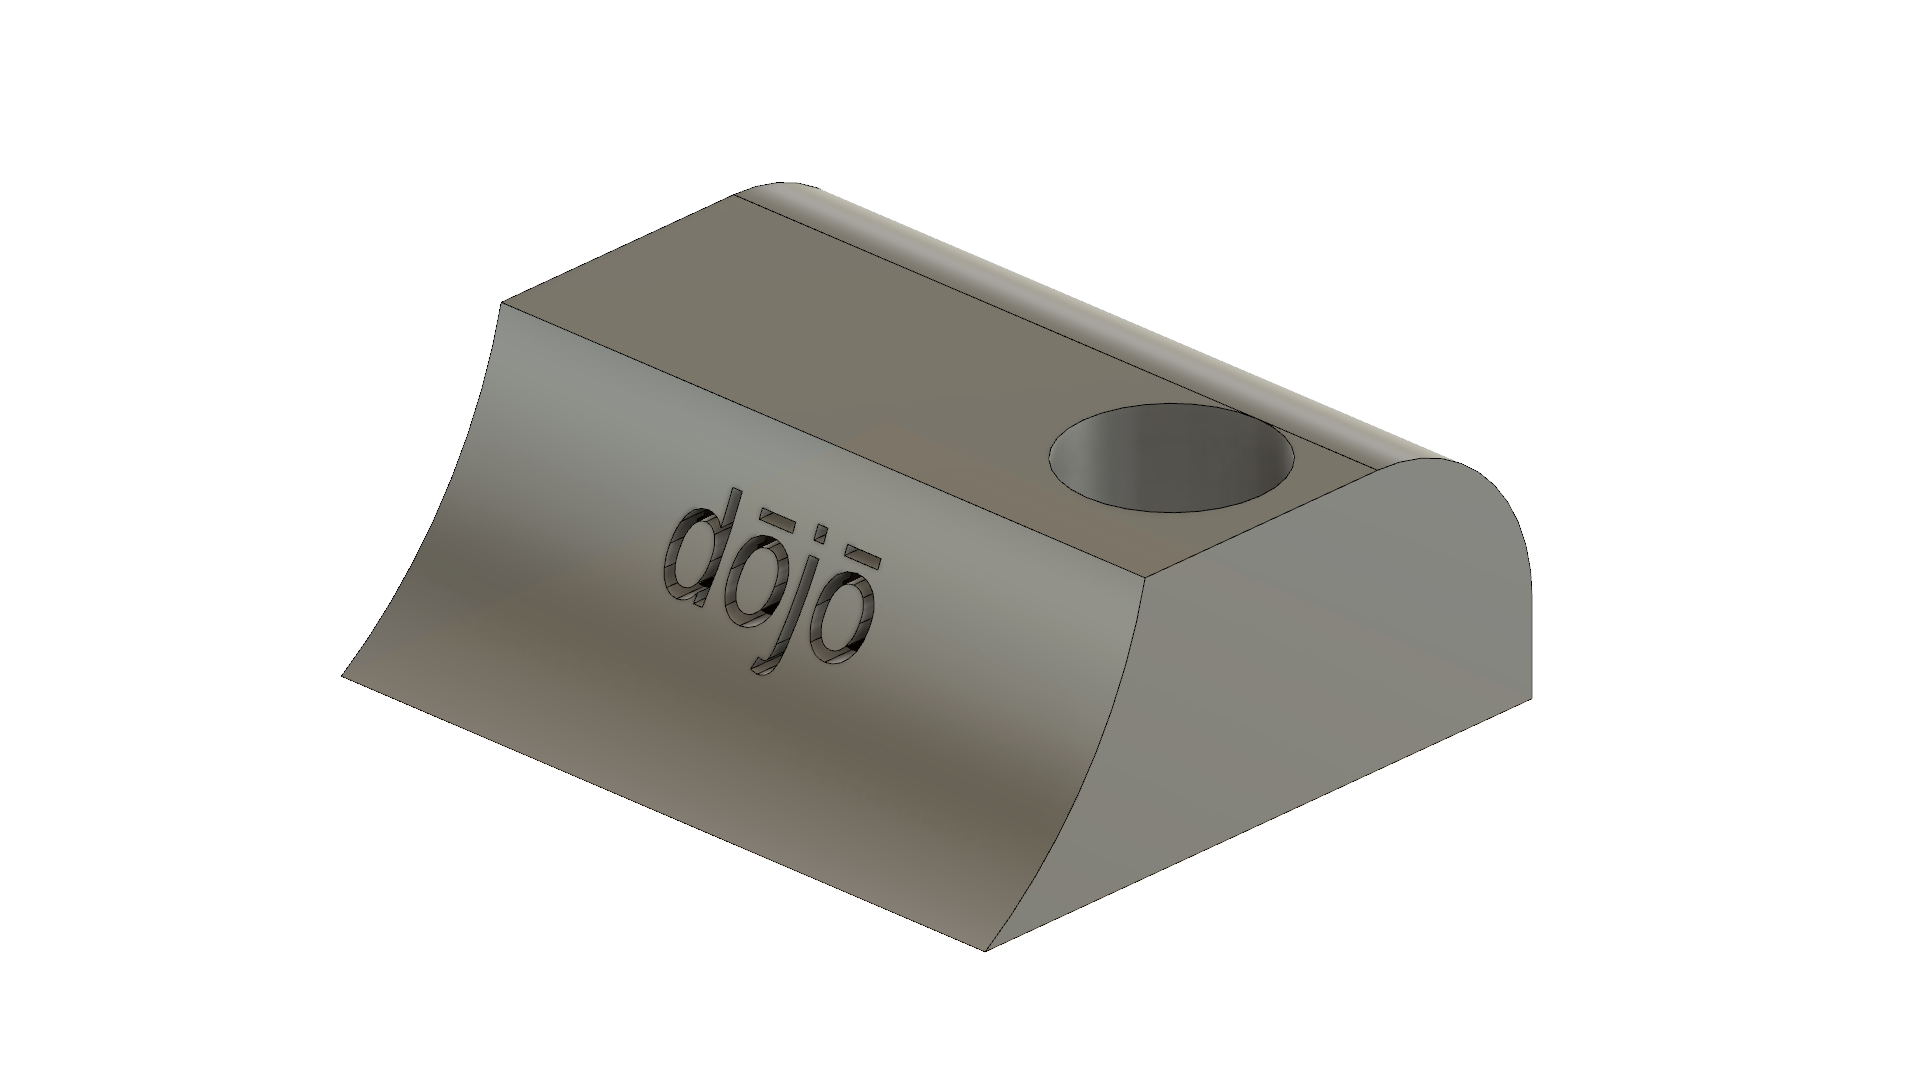
\includegraphics[width=120mm]{data/DojoLadestation01.png}
		\caption[Prototyp Ladestation Frontansicht]{Frontansicht - Ladestation Dojo} %picture caption
		\label{fig:Prototyp Front}
	\end{center}
\end{figure}

Die oben gezeigte Abbildung gibt einen Einblick in das Design von vorne. Augenfällig ist die Öffnung für den Dojo selbst, welche zum einen als Standhalterung und zum anderen als korrekte Positionierung für die induktive Ladeschaltung dient. Weiter ist der Dojo Schriftzug ersichtlich, welcher bis in die dahinter liegende Kammer führt. Die Verwendung wird nachfolgend unter der Abbildung \ref{fig:Prototyp Down} weiter erklärt. 


\begin{figure}[H]
	\begin{center}
		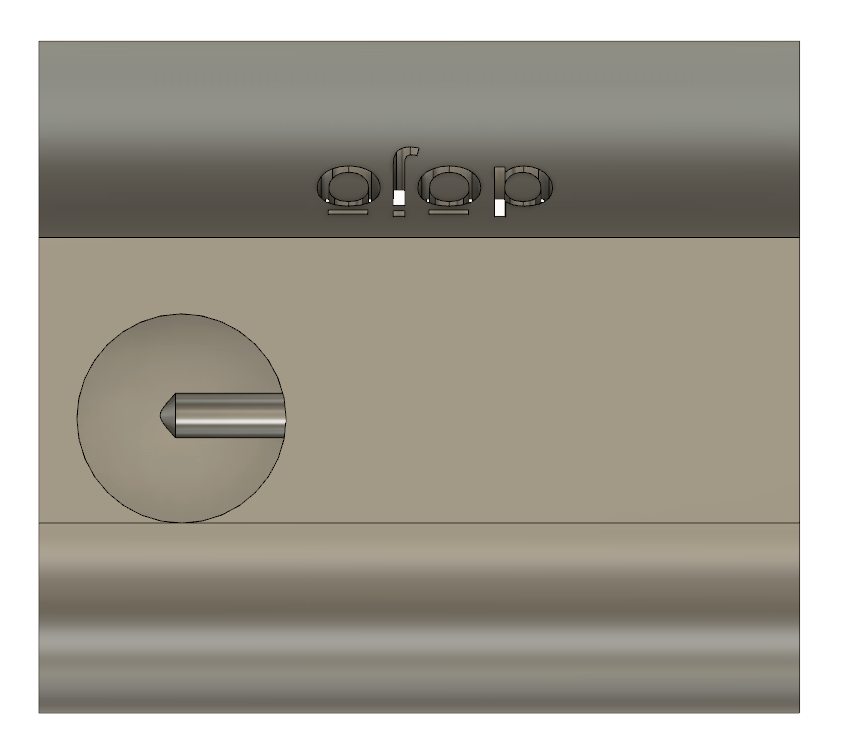
\includegraphics[width=120mm]{data/DojoLadestation02.png}
		\caption[Prototyp Ladestation Draufsicht]{Draufsicht - Ladestation Dojo} %picture caption
		\label{fig:Prototyp Top}
	\end{center}
\end{figure}

Die obige Abbildung \real{fig: Prototyp Top} zeigt den Prototypen von oben. In der Aussparung für den Dojo ist ein Kanal für die Verkabelung der Primärspule ersichtlich. Diese Öffnung führt zur Kammer welche den Primär-Ladekreises beinhaltet. Die Abmessung (Länge x Breite x Höhe) des Prototypen ist (80 x 70.7 x 30)mm.
Nachfolgende Abbildung \ref{fig:Prototyp Down} zeigt den Prototypen von unten.

\begin{figure}[H]
	\begin{center}
		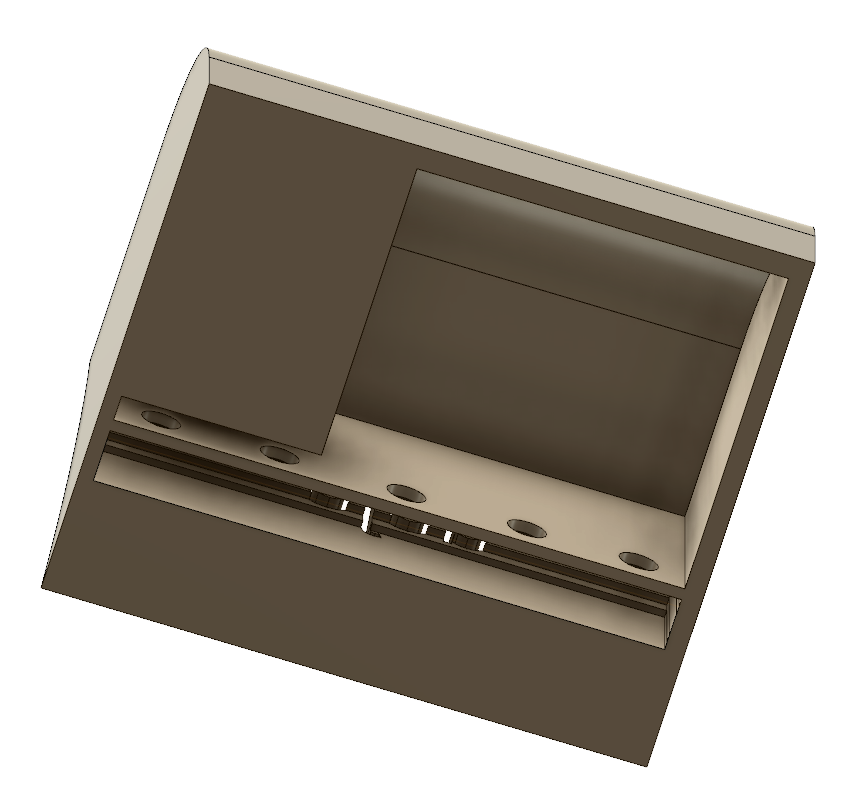
\includegraphics[width=120mm]{data/DojoLadestation03.png}
		\caption[Prototyp Ladestation Ansicht von Unten]{Ansicht von Unten - Ladestation Dojo} %picture caption
		\label{fig:Prototyp Down}
	\end{center}
\end{figure}

Die grosse Kammer ist wie bereits oben beschrieben für den Primärkreis der induktiven Ladeschaltung vorgesehen. Es sind zudem runde 5mm im Durchmesser grosse Löcher ersichtlich welche in die Kammer des Schriftzuges führen ersichtlich. Diese Durchführungen sind für LED vorgesehen, welche den Dojo Schriftzug bei angeschlossener Versorgungsspannung zum Leuchten bringt. 